\chapter{Attosecond Transient-absorption Spectroscopy}
\label{chap:ATS}

\section{Introduction}
\label{sec:intro_ats}

\section{Theory}
\label{sec:atas_theory}

\section{Autoionization resonances}
\label{sec:fano_ar}

One of the most extensively studied phenomenons using ATS has been autoionization of noble gas atoms in the time-domain \cite{wangAttosecondTimeResolvedAutoionization2010, ottAttosecondMultidimensionalInterferometry2012, stoossRealTimeReconstructionStrongFieldDriven2018, kaldunExtractingPhaseAmplitude2014, kaldunObservingUltrafastBuildup2016}.  Autoionization was first observed in 1935 by Beutler \cite{beutlerUeberAbsorptionsserienArgon1935} by studying photoabsorption of noble gas atoms, and it manifested itself as sharp, asymmetric peaks in the absorption spectrum.  These features were theoretically described by Fano in a seminal paper in 1961 \cite{fanoSulloSpettroDi1935, fanoEffectsConfigurationInteraction1961} as the result of interference between two pathways: direct ionization to the continuum and autoionization from a discrete state that is embedded in and coupled to the continuum. The theoretical framework that he developed can be treated as a more general formalism that describes interference between discrete and continuous pathways.\footnote{A very similar theory was independently developed by Feshbach in the context of nuclear physics, and these two theories have been unified by further theoretical work \cite{feshbachUnifiedTheoryNuclear1958, feshbachUnifiedTheoryNuclear1962, bhatiaLineshapeParameters1P1984}
	.} For this very reason, "Fano" resonances can be observed in a plethora of atomic, molecular, and condensed matter systems \cite{miroshnichenkoFanoResonancesNanoscale2010}.

\subsection{Time-independent autoionization: Fano's original work}
\label{sec:og_fano}

As noted above, Fano's theoretical explanation of the photoabsorption spectrum observed by Beutler in noble gas atoms is based on interference between two pathways.  The relevant level diagram to describe this scenario is shown in figure \ref{fig:fano_level_diagram}, and specifically we will be considering the autoionization resonances in Ar because they will be used in the ATS experiments described in this chapter and in the following chapter.  In this case, there is a bound state $\ket{\psi_b}$ (one of the $3s3p^6np$ states in Ar) that is embedded within a set of continuum states $\ket{\psi_\varepsilon}$.  This entails that the energy of the bound state $E_b$ is degenerate with the energetic spectrum of continuum states. The coupling between the bound state $\ket{\psi_b}$ and the continuum $\ket{\psi_\varepsilon}$ through the configuration interaction leads to decay of the electron from the bound state to the continuum.  The following derivation of the photoabsorption cross section and phase follows closely from Fano's original paper and sources that have reproduced his original derivation \cite{fanoEffectsConfigurationInteraction1961, changFundamentalsAttosecondOptics2011, ottAttosecondMultidimensionalInterferometry2012}.

\begin{figure}
	\centering
	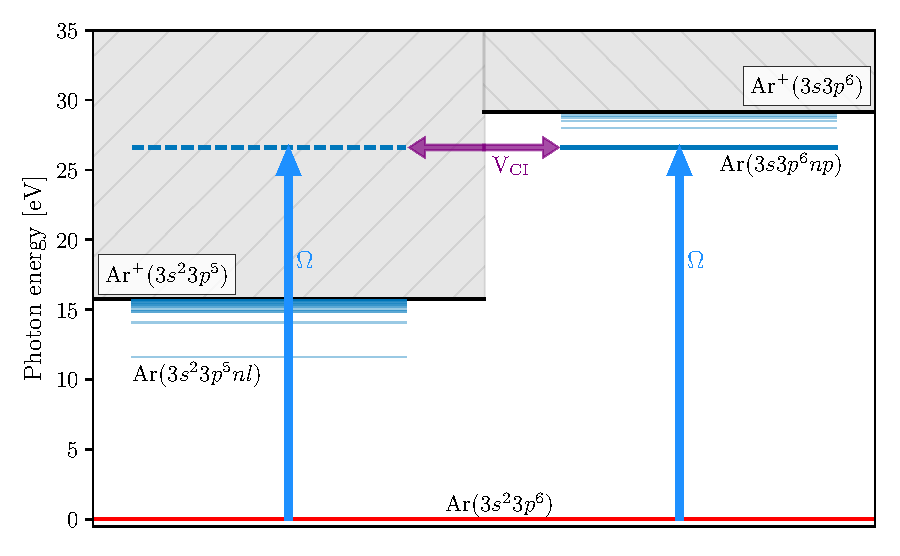
\includegraphics[width=0.8\textwidth]{figures/ATS/fano_level_diagram.pdf}
	\caption{Level diagram of argon showing the effect of autionization states on XUV photoabsorption. There are two possible pathways for ionization with a photon of energy $\Omega$: (1) direct ionization to a continuum state (left side of figure) and (2) excitation to a bound state in the continuum (right side of figure).  In case (2), there is coupling between the bound state and the continuum through the configuration interaction.  This allows for the bound state to decay to the same contiuum state as in case (1).  These effect leads to interference between these two pathways.}
	\label{fig:fano_level_diagram}
\end{figure}

The Hamiltonian describing this system can  be written as
\begin{equation}
\label{eqn:hamiltonian}
	\hat{H} = \hat{H_0} + \hat{V},
\end{equation}
where $\hat{H_0}$ is the zeroth order Hamiltonian and $\hat{V}$ is the correlation potential that describes the coupling between the discrete state $\ket{\psi_b}$ and the continuum state $\ket{\psi_\varepsilon}$.  The solutions to the zeroth order Hamiltonian are the continuum and bound states, such that 
\begin{align}
\label{eqn:configurations_hamiltonian}
	\hat{H_0}\ket{\psi_b} &= E_b\ket{\psi_b}\\
	\hat{H_0}\ket{\psi_\varepsilon} &= \varepsilon\ket{\psi_\varepsilon}
\end{align}
where the states $\ket{\psi_b}$ and $\ket{\psi_\varepsilon}$ are orthonormal.  These two solutions to the zeroth order Hamiltonian are referred to as configurations, and the interaction between them is given by $\hat{V}$. The coupling strength between these two configurations is given by the off-diagonal matrix element $V_\varepsilon$, such that
\begin{equation}
\label{eqn:coupling_matrix_element}
	\braket{\psi_\varepsilon|\hat{H}|\psi_b} = \braket{\psi_\varepsilon|\hat{H_0}+\hat{V}|\psi_b} = \braket{\psi_\varepsilon|\hat{V}|\psi_b} = V_\varepsilon.
\end{equation}  
This configuration interaction matrix element $V_\varepsilon$ depends upon the energy $\varepsilon$ and is generally a smooth function of the continuous energy $\varepsilon$.  Furthermore, the configuration interaction only couples different configurations and not within the same configuration.  The means that the diagonal matrix elements of $\hat{V}$ are zero,
\begin{align}
\label{eqn:config_int_diagonal}
	\braket{\psi_\varepsilon|\hat{V}|\psi_\varepsilon} &=0\\
	\braket{\psi_b|\hat{V}|\psi_b} &=0.
\end{align}
Therefore, the diagonal matrix elements of the full Hamiltonian in equation \ref{eqn:hamiltonian} are given by
\begin{align}
	\braket{\psi_\varepsilon|\hat{H}|\psi_\varepsilon} &= \varepsilon\delta(\varepsilon-\varepsilon')\\
	\braket{\psi_b|\hat{H}|\psi_b} &= E_b. 
\end{align}

Armed with these states as a basis, we can now expand an eigenstate of the full Hamiltonian $\hat{H}$.  This entails that the eigenstate $\ket{\Psi_E}$ of energy $E$, which is found by solving the equation
\begin{equation}
	\hat{H}\ket{\Psi_E}=E\ket{\Psi_E},
\end{equation}
can be expanded in this complete basis, such that
\begin{equation}
\label{eqn:eigenstate_expansion}
	\ket{\Psi_E} = a(E)\ket{\psi_b} + \int\diff\varepsilon'b(\varepsilon',E)\ket{\psi_{\varepsilon'}}.
\end{equation}
The physical interpretation of this expansion is that an electron at energy $E$ can originate from either the discrete state $\ket{\psi_b}$ or from the continuous state $\ket{\psi_\varepsilon}$.  The contribution from $\ket{\psi_\varepsilon}$ is direct ionization, and the contribution from $\ket{\psi_b}$ is autoionization (i.e. decay from the bound state $\ket{\psi_b}$ to the continuum).  The relative contributions of these two channels is given by the expansion coefficients $a(E)$ and $b(\varepsilon,E)$.

These expansion coefficients can be solved for and it involves algebra that is described in full detail in Fano's paper \cite{fanoEffectsConfigurationInteraction1961}.  The first step is to evaluate the relationship
\begin{equation}
	\braket{\Psi_E|\hat{H}|\Psi_E} = E
\end{equation}
using the expansion in eqn. \ref{eqn:eigenstate_expansion}.  This results in a system of two equations with the unknown coefficients $a(E)$ and $b(\varepsilon,E)$.  This system can be solved for analytical expressions of the expansion coefficients, and they are given by
\begin{align}
\label{eqn:expansion_coeff_a}
	a(E) &= \frac{\sin\Delta(E)}{\pi V_E}\\
\label{eqn:expansion_coeff_b}
	b(\varepsilon',E) &= \frac{V_{\varepsilon'}}{E-\varepsilon'}a(E)-\delta(\varepsilon'-E)\cos\Delta(E)
\end{align}
where
\begin{align}
\label{eqn:expansion_coeff_delta_F}
	\Delta(E) &= -\arctan\bigg(\frac{\pi\lvert V_E \rvert^2}{E-E_b-F(E)}\bigg)\\
	F(E) &= \mathrm{PV}\int\diff\varepsilon'\frac{\lvert V_{\varepsilon'}\rvert^2}{E-\varepsilon'} 
\end{align}
and $\mathrm{PV}$ is the Cauchy principal value. The term  $F(E)$ is an energy-dependent shift of the bound state that depends upon the strength of the configuration interaction $\abs{V_{\varepsilon'}}^2$.  This shift can be either positive or negative, depending upon the sign of $\partial_{\varepsilon'}\abs{V_{\varepsilon'}}^2$ at $\varepsilon'=E$, where $\partial_{\varepsilon'}$ is the partial derivative with respect to $\varepsilon'$.  Thus, any change in  $V_{\varepsilon'}$ by an external field will lead to a shift in the resonance position.

Substituting the coefficients in equations \ref{eqn:expansion_coeff_a} and \ref{eqn:expansion_coeff_b} into equation \ref{eqn:eigenstate_expansion} yields
\begin{equation}
	\ket{\Psi_E}=\frac{\sin\Delta(E)}{\pi V_E}\ket{\psi_b}+\frac{\sin\Delta(E)}{\pi V_E}\bigg(\mathrm{PV}\int\diff\varepsilon'\frac{V_{\varepsilon'}}{E-\varepsilon'}\bigg)\ket{\psi_\varepsilon'}-\cos\Delta(E)\ket{\psi_E}.
\end{equation}
This can be further simplified by  introducing a modified discrete state given by
\begin{equation}
	\ket{\Phi} = \ket{\psi_b}+\mathrm{PV}\int\diff \varepsilon'\frac{V_\varepsilon'}{E-\varepsilon'}\ket{\psi_{\varepsilon'}}.
\end{equation}
Finally, the eigenstate $\ket{\Psi_E}$ can be expressed as
\begin{equation}
	\ket{\Psi_E}=\frac{\sin\Delta(E)}{\pi V_{E}}\ket{\Phi} - \cos\Delta(E)\ket{\psi_E}.
\end{equation}


\begin{figure}
	\centering
	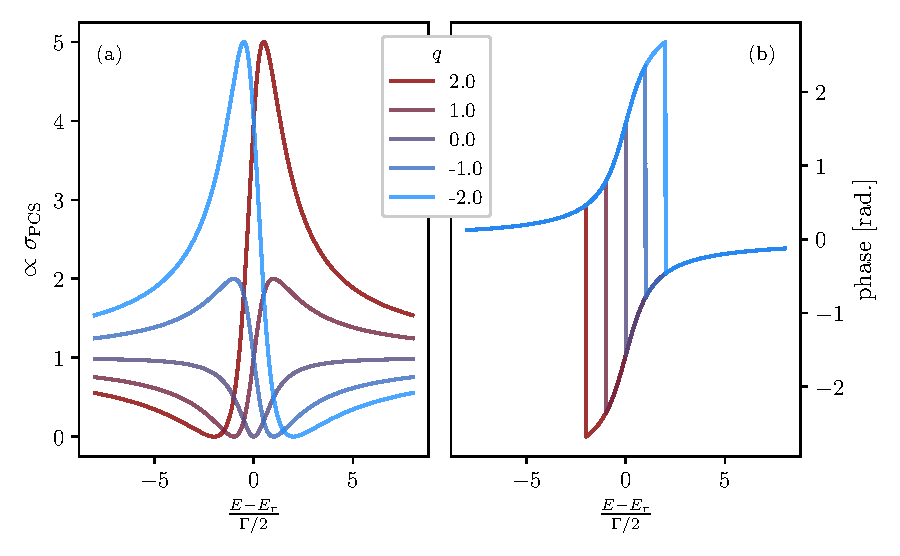
\includegraphics[width=0.9\textwidth]{figures/ATS/cs_phase.pdf}
	\caption{(a) Calculation of the photoabsorption cross section near a resonance for the listed $q$ parameters.  The change from symmetric to antisymmetric profiles can be seen as the $q$ parameter is varied. (b) Calculation of the phase across the resonance for different $q$ parameter. The $\pi$ phase jump clearly depends on $q$, and it occurs when $\epsilon=-q$ and not at the resonance energy $E_r$. Calculations based on U. Fano's original work \cite{fanoEffectsConfigurationInteraction1961}.}
	\label{fig:cross_sec_and_phase}
\end{figure}

\begin{table}[]
	\centering
	\begin{tabular}{lcccc}
		\hline\hline
		\multicolumn{1}{c}{} & $\Delta E$ [eV]   & $\Gamma$ [meV]   & $q$         & $\rho^2$     \\ \hline
		$3s3p^64p$              & 26.605 & 80.2(7) & -0.286(4) & 0.840(3) \\
		$3s3p^65p$              & 27.994 & 28.5(8) & -0.177(3) & 0.848(3) \\
		$3s3p^66p$              & 28.509 & 12.2(3) & -0.135(9) & 0.852(9) \\
		$3s3p^67p$              & 28.757 & 6.6(1)  & -0.125(4) & 0.846(9) \\
		$3s3p^68p$              & 28.898 & 4.5(2)  & -0.132(4) & 0.77(2)  \\ \hline\hline
	\end{tabular}
	\caption{Paramters of the $3s3p^6np$ Fano resonances in argon. These values were extracted from experimental cross sections, see \cite{caretteMulticonfigurationalHartreeFockClosecoupling2013}.}
	\label{table:fano_params}
\end{table}


\begin{figure}
	\centering
	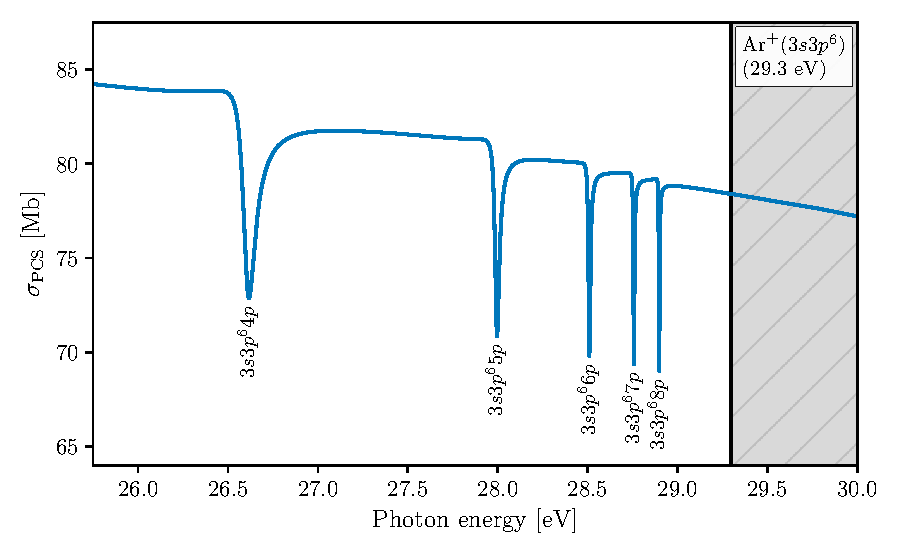
\includegraphics[width=0.8\textwidth]{figures/ATS/fano_GS.pdf}
	\caption{Photoabsorption cross section of the Argon $3s3p^6np$ Fano resonances (blue curve), with only resonances up to $n=8$ shown.  Grey shaded area indicates the energetic region above the $\mathrm{Ar}^+(3s3p^6)$ ionization threshold. Values used to calculate this cross section are shown in Table \ref{table:fano_params}.}
	\label{fig:fano_gs_pcs}
\end{figure}

\begin{figure}
	\centering
	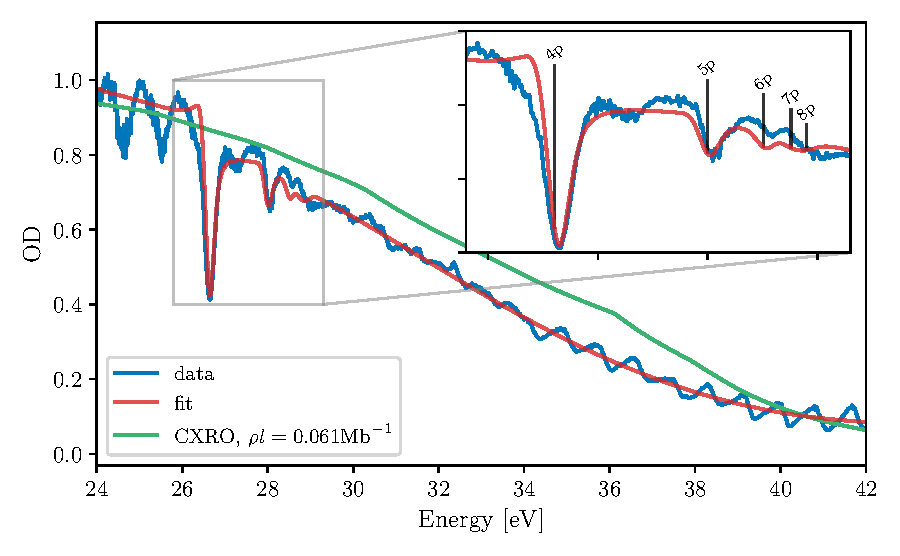
\includegraphics[width=0.8\textwidth]{figures/ATS/fano_fit.pdf}
	\caption{Incomplete}
	\label{fig:fano_fit}
\end{figure}

\subsection{Time-dependent autoionization}

\section{Strong-field Transient Absorption in Argon}
\label{sec:ATS_ar}

\subsection{Experimental setup}
\label{sec:ATS_ar_exp_setup}

\subsection{Results}
\label{sec:ATS_ar_results}

\section{Conculsion}
\label{sec:ATS_conclusion}

